\documentclass[tikz]{standalone}
\usepackage{xparse}
\colorlet{curveZero}{gray!75}
\colorlet{curveOne}{blue!60}
\colorlet{curveTwo}{brown!50!gray}
\colorlet{curveThree}{green!40!gray}
\colorlet{curveFour}{red!50!gray}
\NewDocumentCommand\DrawDotInPlot{O{}mmO{}}%
{%
\fill[gray!20,draw=gray] (axis cs:{#2},{#3}) circle (1.3pt) node[above,black,#4] {\(#1\)};%
}%
\NewDocumentCommand\DrawDot{O{}mmO{}}%
{%
\fill[gray!20,draw=gray] ({#2},{#3}) circle (1.3pt) node[above,black,#4] {\(#1\)};%
}%
\NewDocumentCommand\DrawNode{O{}m}%
{%
\fill[gray!20,draw=gray] (#2) circle (1.3pt) node[above,black] {\(#1\)};%
}%
\colorlet{axisColor}{gray!50}
\tikzstyle{shapeZero}=[fill=curveZero,opacity=.4]
\tikzstyle{shapeOne}=[fill=curveOne,opacity=.4]
\tikzstyle{shapeTwo}=[fill=curveTwo,opacity=.4]
\tikzstyle{shapeThree}=[fill=curveThree,opacity=.4]
\tikzstyle{groupElementLabel}=[minimum size=2.4em]
\tikzstyle{groupElement}=[minimum size=2.4em,shapeZero,draw=curveZero]
\tikzstyle{cosetOne}=[minimum size=2.4em,shapeOne,draw=curveOne]
\tikzstyle{cosetTwo}=[minimum size=2.4em,shapeTwo,draw=curveTwo]


\begin{document}
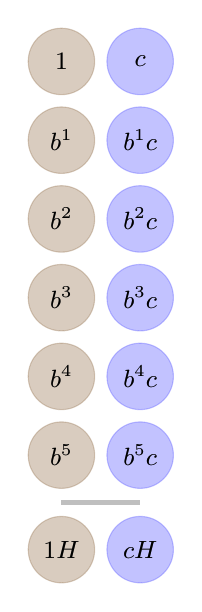
\begin{tikzpicture}
\newcommand{\Radiii}{1}
        \foreach \x in {1,...,5} {
                \node[circle,cosetOne] 
                at (1,{-\Radiii*\x}) 
                {\small\(b^{\x}c\)};
                \node[circle,groupElementLabel] 
                at (1,{-\Radiii*\x}) 
                {\small\(b^{\x}c\)};
                \node[circle,cosetTwo] 
                at (0,{-\Radiii*\x}) 
                {\small\(b^{\x}\)};
                \node[circle,groupElementLabel] 
                at (0,{-\Radiii*\x}) 
                {\small\(b^{\x}\)};
		}
        \node[circle,cosetOne] at (1,0) {\small\(c\)};
        \node[circle,groupElementLabel] at (1,0) {\small\(c\)};
        \node[circle,cosetTwo] at (0,0) {\small\(1\)};        
        \node[circle,groupElementLabel] at (0,0) {\small\(1\)};        
        \draw [axisColor,ultra thick] (0,{-\Radiii*5.6}) -- (1,{-\Radiii*5.6});
        \node[circle,cosetOne] at (1,{-\Radiii*6.2}) {\small\(cH\)};
        \node[circle,groupElementLabel] at (1,{-\Radiii*6.2}) {\small\(cH\)};
        \node[circle,cosetTwo] at (0,{-\Radiii*6.2}) {\small\(1H\)};        
        \node[circle,groupElementLabel] at (0,{-\Radiii*6.2}) {\small\(1H\)};       
\end{tikzpicture}
\end{document}
